%%%%%%%%%%%%%%%%%%%%%%%%%%%%%%%%%%%%%%%%%%%%%%%%%%%%%%%%%%%%%%%%%%%%%%%%%%%%%%%%
%2345678901234567890123456789012345678901234567890123456789012345678901234567890
%        1         2         3         4         5         6         7         8

\documentclass[letterpaper, 9 pt, conference]{ieeeconf}  % Comment this line out if you need a4paper

%\documentclass[a4paper, 11pt, conference]{ieeeconf}      % Use this line for a4 paper

\IEEEoverridecommandlockouts                              % This command is only needed if 
                                                          % you want to use the \thanks command

\overrideIEEEmargins                                      % Needed to meet printer requirements.

% See the \addtolength command later in the file to balance the column lengths
% on the last page of the document

% The following packages can be found on http:\\www.ctan.org
%\usepackage{graphics} % for pdf, bitmapped graphics files
%\usepackage{epsfig} % for postscript graphics files
%\usepackage{mathptmx} % assumes new font selection scheme installed
%\usepackage{times} % assumes new font selection scheme installed
%\usepackage{amsmath} % assumes amsmath package installed
%\usepackage{amssymb}  % assumes amsmath package installed
\usepackage{graphicx}
\usepackage{hyperref}
\usepackage{verbatim}
\title{\LARGE \bf
Exploration and Mapping with a Particle Swarm\\ Controlled by Uniform Inputs on a Magnetic Setup
}


\author{Daniel Bao, Arun Mahadev, Aaron T. Becker% <-this % stops a space
\thanks{D. Bao, A.~Mahadev, and A.~Becker are with the Department of Electrical and Computer Engineering,  University of Houston, Houston, TX 77204-4005 USA 
      \protect\url{dzbao@uh.edu,aviswanathanmahadev@uh.edu,atbecker@uh.edu }}
\thanks{*This work was supported by the National Science Foundation under Grant No.\ \href{http://nsf.gov/awardsearch/showAward?AWD_ID=1553063}{ [IIS-1553063]} and \href{http://nsf.gov/awardsearch/showAward?AWD_ID=1619278}{[IIS-1619278]}.}% <-this % stops a space
}
\begin{document}



\maketitle
\thispagestyle{empty}
\pagestyle{empty}


%%%%%%%%%%%%%%%%%%%%%%%%%%%%%%%%%%%%%%%%%%%%%%%%%%%%%%%%%%%%%%%%%%%%%%%%%%%%%%%%
\section{Introduction}\label{sec:Introduction}
	This research deals with mapping a workspace using a swarm of non-intelligent robots or particles. Much work has been done in single robot mapping, but there is a gap of research for multiple robots exploring an environment using the same input commands, also known as global uniform control. In our previous work~\cite{AAM}, we developed a ClosestFrontier algorithm, with frontiers being unknown boundary cells, that maps a discrete 2D workspace using global uniform control. Here we expand its scope to 3D environments, implement a physical hardware setup using four orthogonal magnetic coils, and develop a ROS simulation using MATLAB's Robotic Toolbox.
\section{Methods and Results}\label{sec:Methods and Results}
	For the physical setup, we use resin-bound acrylic to create a transparent workspace compatible with the black paramagnetic particles suspended on the water's surface and a camera recording from below (See Fig. 3). This allows for more dynamic interactions as well as continuous boundaries. New challenges like wall friction, surface tension, and  hydrophobic interactions between the particles now arise from the physicality of the setup. These physical properties prove hardest to overcome in small branched maps because of the steep meniscus and local minimum of water that the particles face. To address this problem, we designed our workspaces with optimized channel width and curved edges to avoid local minimums.
	
	Expanding the previous 2D simulation to 3D required us to increase the matrix dimensions and the nodes required to search with the ClosestFrontier algorithm but the extra dimension didn't require more moves to completely map the workspace when the free space count was the same. More simply, there is no trade-off between dimensions and moves required to completely map the explored workspace. Only the complexity of the map matters, which means that for the same number of free spaces on a 2D and 3D map, the map with the more complex shape will require more total moves to map with the ClosestFrontier algorithm. Complex shapes are highly branched and take many turns and loops which makes mapping longer. Examples are shown in Fig. 1 and 2.
	
	Upgrading the simulation required fundamental changes within the program that now uses the Robotics Toolbox in MATLAB that enables continuous workspaces. This toolbox allows ROS, or Robotics Operating System, integration with MATLAB object oriented programming and scripts. The new simulator consists of a class instantiating \textit{n} robots in a workspace defined by a image file. The difference is that this simulation uses low-range distance sensors to simulate the boundary interactions instead of comparing position data after inputs. An occupancy grid allows for scanning and moving.
\section{Discussion}\label{sec:Discussion}
	This research allows for precise control over weaker para-magnetic particles as well as a theoretical understanding of algorithmic efficiency in real world workspaces. Ultimately, medicinal applications in active targeted drug delivery and mapping vasculature as an alternative to traditional contrast agents are fields that can benefit from this research as well as more studies on non-invasive particle treatments. 
\begin{figure}
	%\vspace{-20pt}
\begin{comment}
	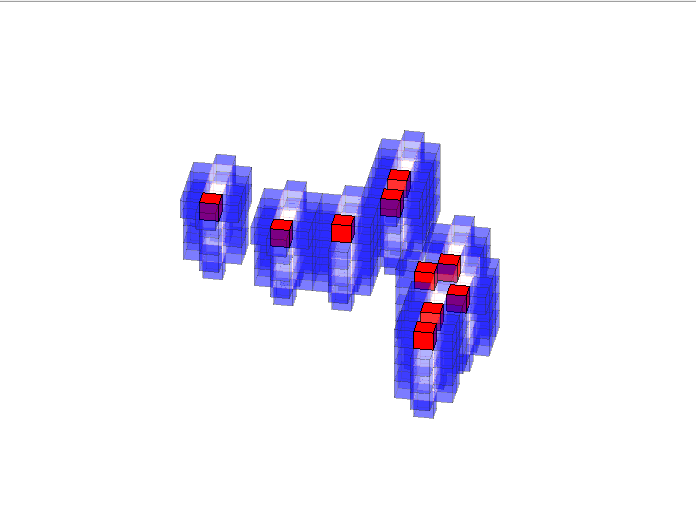
\includegraphics[height=0.2\paperheight]{3d1.png}
	\caption{The 3D simulation is shown above with red blocks being the particles, blue being the frontier cells, and white being free explored cells.}
\end{comment}
	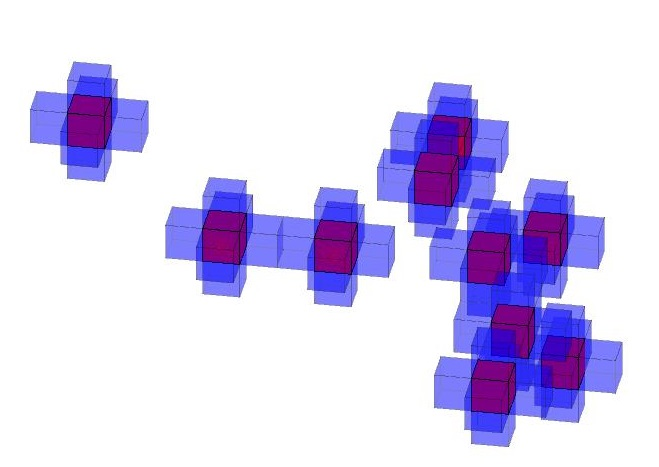
\includegraphics[width=0.15\textwidth]{3D_initial}
	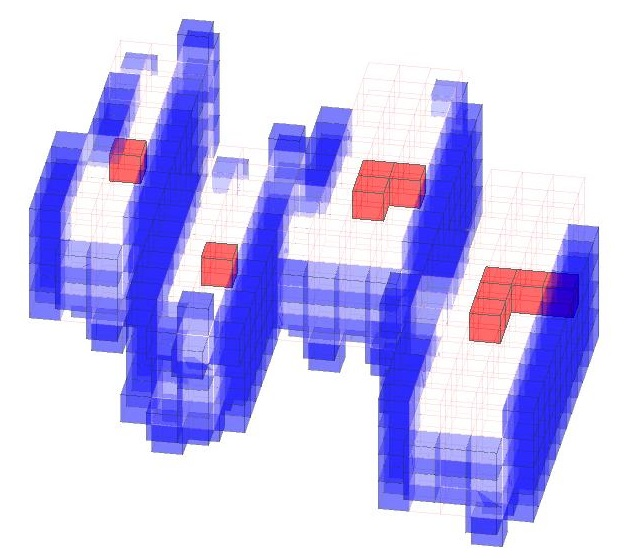
\includegraphics[width=0.15\textwidth]{3D_middle}
	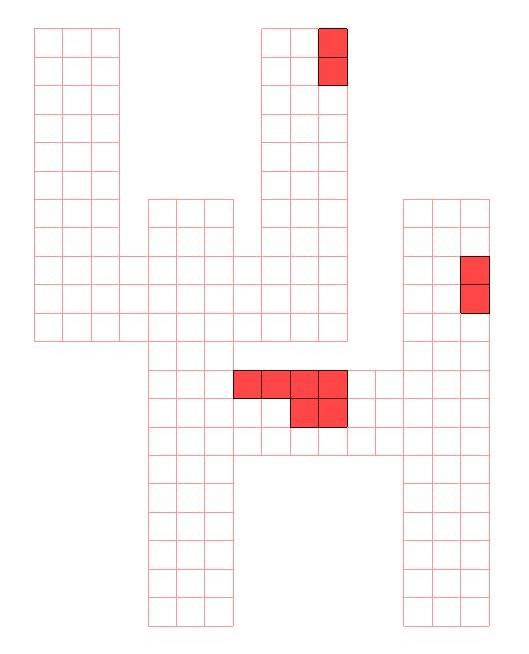
\includegraphics[width=0.1\textwidth]{3D_final}
	\caption{Each picture is a snapshot of the 3D mapping process at different stages from initialization to completion. The white blocks are the mapped free spaces and everything else is an obstacle. The mapped workspace is the logo of the University of Houston and has 720 free spaces. This takes around 700-800 moves depending on the initial positions of the particles.}
\begin{comment}
	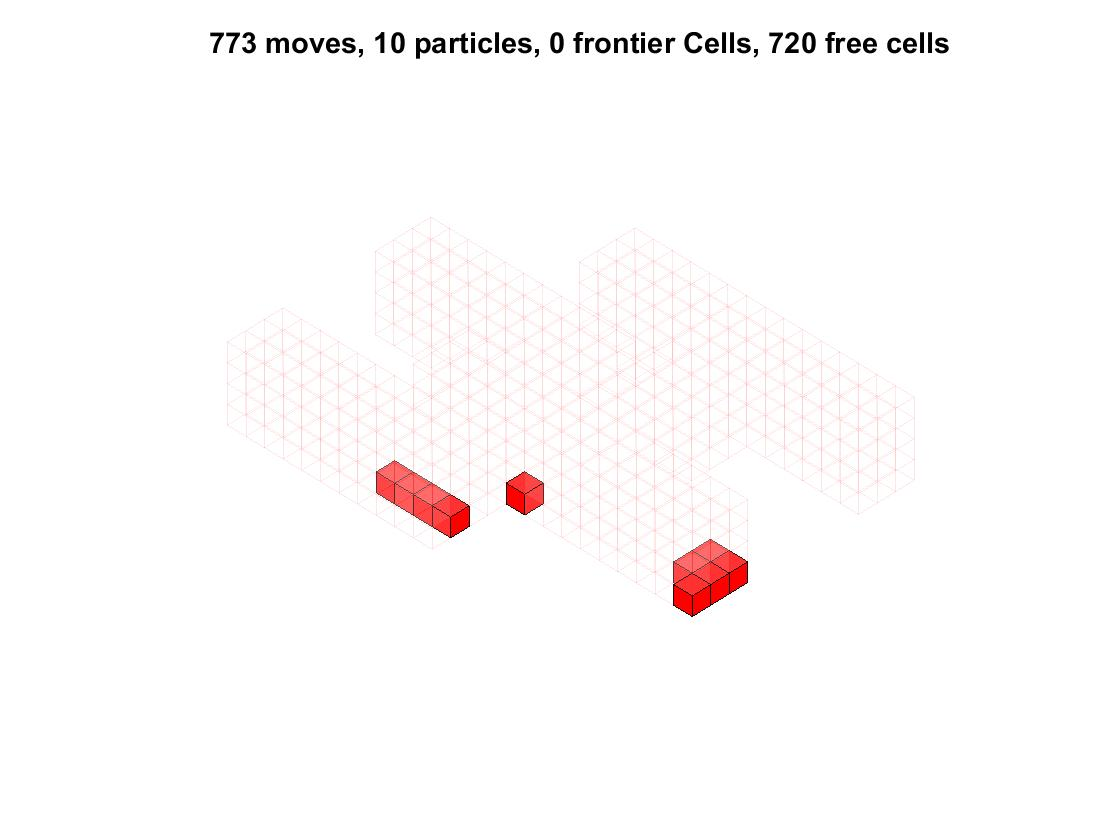
\includegraphics[height=0.18\paperheight]{10particles_3D.jpg}
	\caption{This is another perspective of the completed workspace in Fig. 1. There are four layers for the particles to explore.}
\end{comment}
	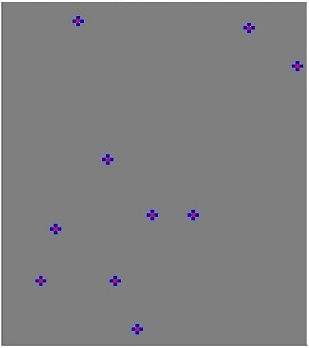
\includegraphics[width=0.1\paperheight]{2D_720_initial.jpg}
	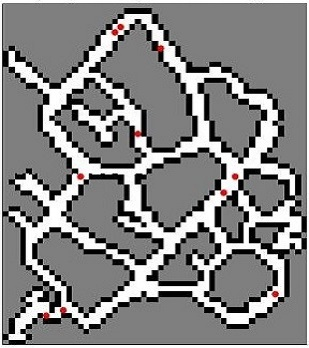
\includegraphics[width=0.1\paperheight]{10particles_final.jpg}
	
	\caption{From left to right, the mapping of this 2D workspace is depicted. For an equivalent number of free cells in 2D, more moves (1100-1200 moves compared to 700-800) were required due to the increased complexity of this vascular system based off of a leaf tissue sample. The 2D simulation uses black blocks to represent boundary cells.}
	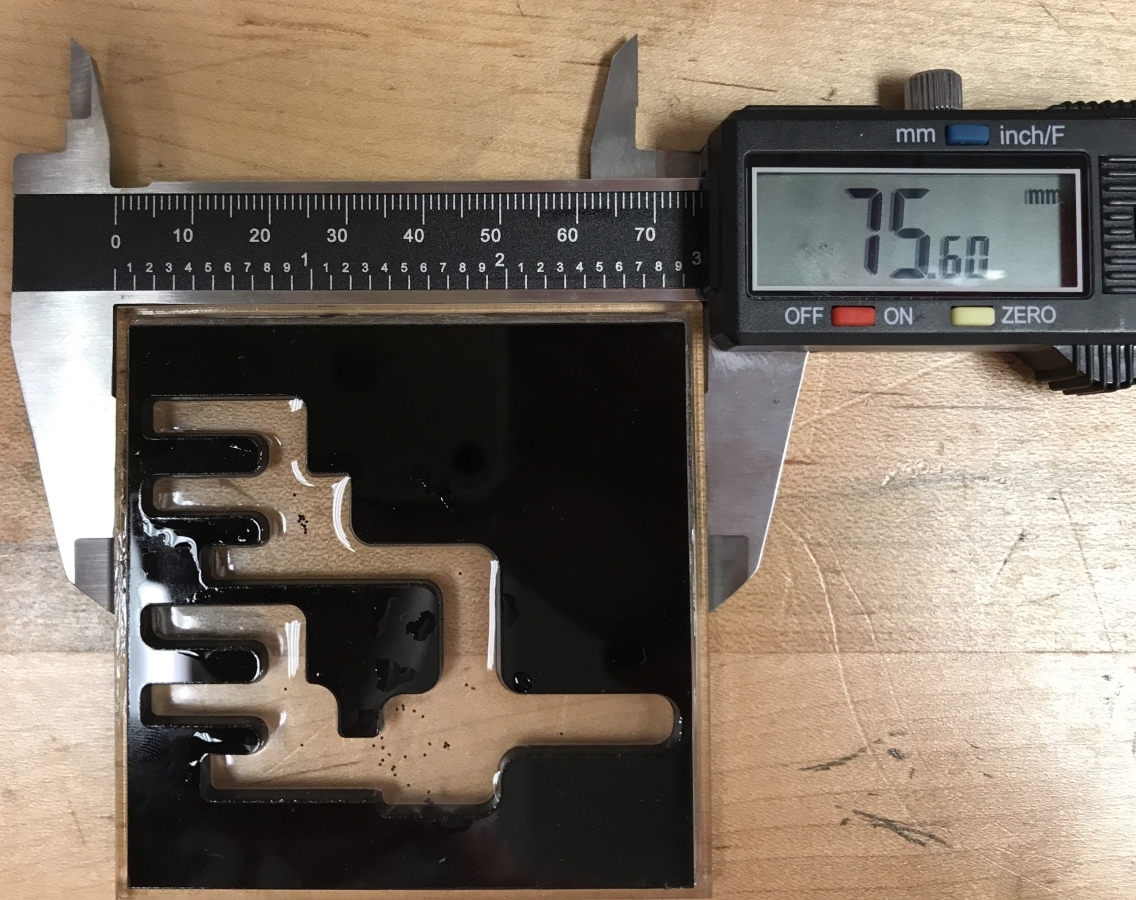
\includegraphics[height=0.10\paperheight]{Optimized-Workspace.jpg}
\caption{
This is a picture of the smoothed out workspace created with acrylic. The small black dots are the paramagnetic particles and they have a diameter of .325 to .455 mm. 
}
\end{figure}
\bibliographystyle{IEEEtran}
\bibliography{abstract}

\end{document}
